%LTeX: language=DE
\chapter{Externe Referenzen}
	\begin{figure}[h]
		\centering
		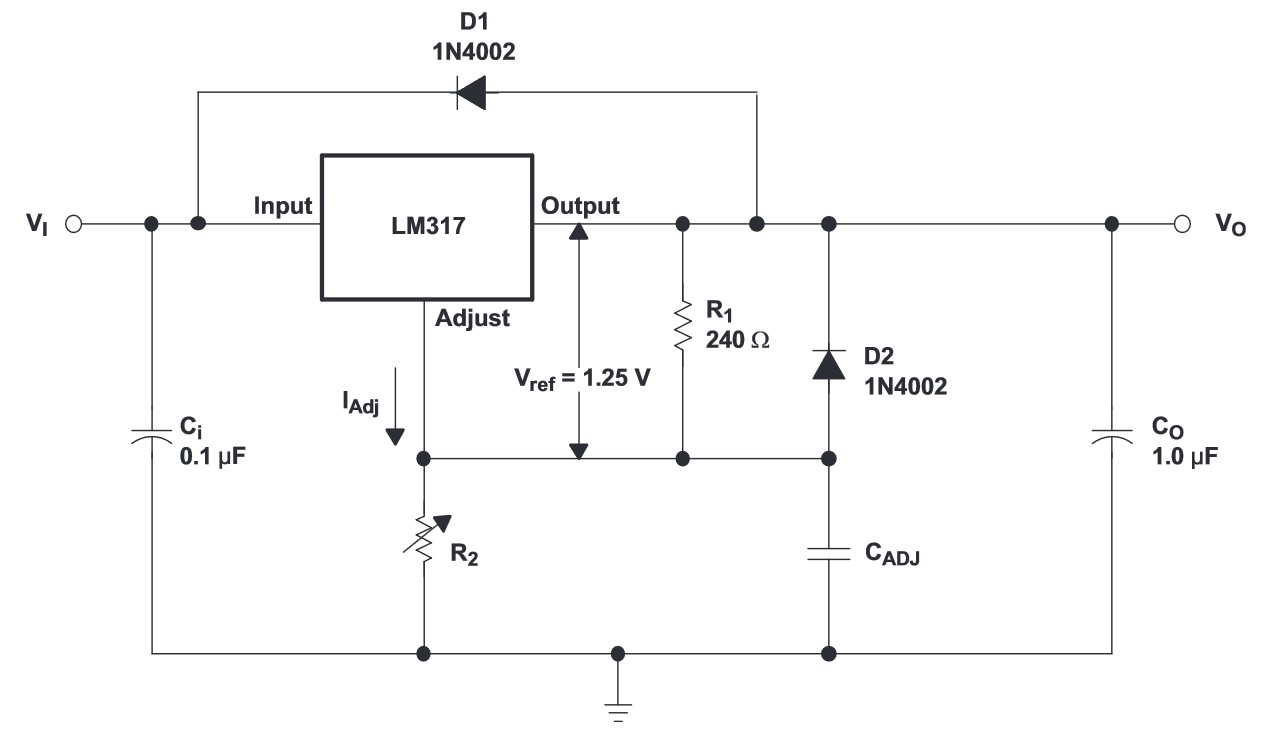
\includegraphics[width=.9\textwidth]{referenzen/typical_app_schem.jpg}
		\caption[Aus dem Datenblatt übernommenes Diagram eines \textit{typischen Anwendungsszenarios} des LM317]{Aus dem Datenblatt übernommenes Diagram
		eines \textit{typischen Anwendungsszenarios} des LM317 Linearreglers \cite{datasheet.LM317.TexasInstruments.2021}. Zentrale Elemente sind hier der Linearregler selbst, sowie
		die beiden Widerstände \(R_1\) und \(R_2\). \(R_2\) insbesondere dient hier zur justierung der Ausgangsspannung.}
		\label{fig:typical app sch}
	\end{figure}
	\newpage
	\begin{figure}[h]
		\centering
		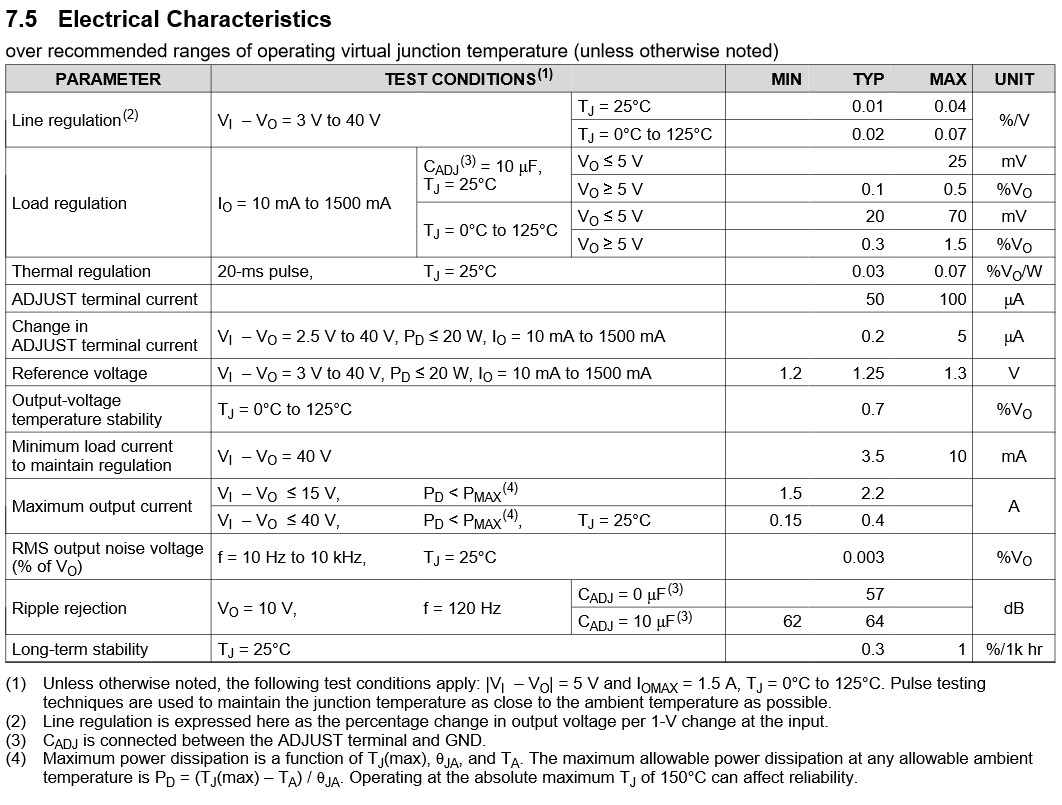
\includegraphics[width=\textwidth]{referenzen/electrical_characteristics_LM317.jpg}
		\caption[Auszug aus dem Datenblatt des LM317 von \textsc{Texas Instruments}]{Auszug aus dem Datenblatt des LM317 von \textsc{Texas Instruments} \cite{datasheet.LM317.TexasInstruments.2021}.}
		\label{tab:lm317 characteristics}
	\end{figure}
	\begin{figure}
		\centering
		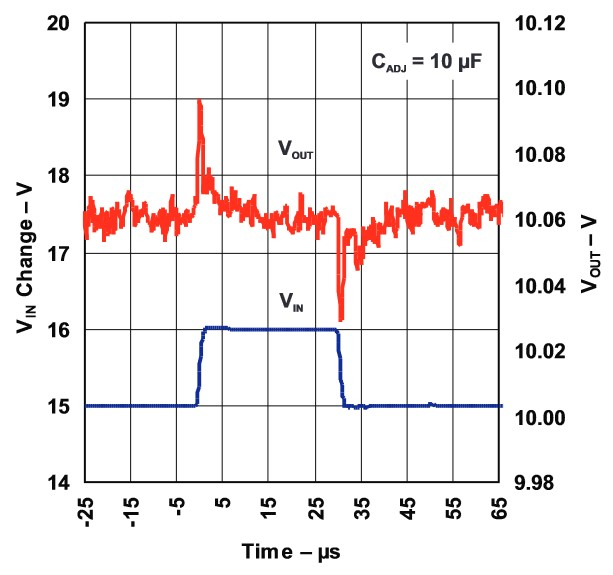
\includegraphics[width=.7\textwidth]{referenzen/line-transient-regulation.jpg}
		\caption[\textit{Line-transient response} aus Kapitel 9.2.3 des Datenblattes zum LM317 von \textsc{Texas Instruments}]{\textit{Line-transient response} aus Kapitel 9.2.3 des Datenblattes zum LM317 von \textsc{Texas Instruments} \cite{datasheet.LM317.TexasInstruments.2021}.}
		\label{fig:line transient response}
	\end{figure}